\documentclass{article}
\usepackage[sfdefault]{FiraSans}
\usepackage[T1]{fontenc}
\usepackage[utf8]{inputenc}
\usepackage{algorithm}
\usepackage{algorithmic}
\usepackage{amsfonts}
\usepackage{amsmath}
\usepackage{amssymb}
\usepackage{booktabs}
\usepackage{float}
\usepackage{geometry}
\usepackage{graphicx}
\usepackage{hyperref}
\usepackage{microtype}
\usepackage{indentfirst}
\usepackage{lipsum}
\usepackage{longtable}
\usepackage{multirow}
\usepackage{natbib}
\usepackage{pdfpages}
\usepackage{setspace}
\usepackage{subcaption}
\usepackage{tabularx}
\usepackage{tikz}
\usepackage{xcolor}

\setlength{\parindent}{0.5in}

% color scheme
\definecolor{primary}{RGB}{0,120,215}
\definecolor{secondary}{RGB}{255,87,34}
\definecolor{background}{RGB}{245,245,245}

% page layout
\geometry{
    letterpaper,
    left=1in,
    right=1in,
    top=1in,
    bottom=1in,
}

% hyperlink colors
\hypersetup{
    colorlinks=true,
    linkcolor=primary,
    filecolor=secondary,
    urlcolor=primary,
}

% page color
\pagecolor{background}

\begin{document}

\setstretch{1.15}
\definecolor{blue}{RGB}{0,62,126}

\newcommand{\mytitlepage}[2]{
    \thispagestyle{empty}

    \begin{tikzpicture}[remember picture, overlay]
        \node [inner sep=0pt] at (current page.center) {#1};
        {
        \node [
            anchor=center,
            inner sep=1.25cm,
            rectangle,
            fill=blue!70!white,
            fill opacity=0,
            text opacity=1,
            minimum height=0.2\paperheight,
            minimum width=\paperwidth,
            text width=0.8\paperwidth,
            font=\fontfamily{pnc}\selectfont
        ] at (current page.center) {#2};
        }
        \node [anchor=south east, outer sep=3pt] at (current page.south east)
        {\includegraphics[width=0.33\paperwidth]{images/logo.png}};
    \end{tikzpicture}

    \newpage
}

{
    \mytitlepage{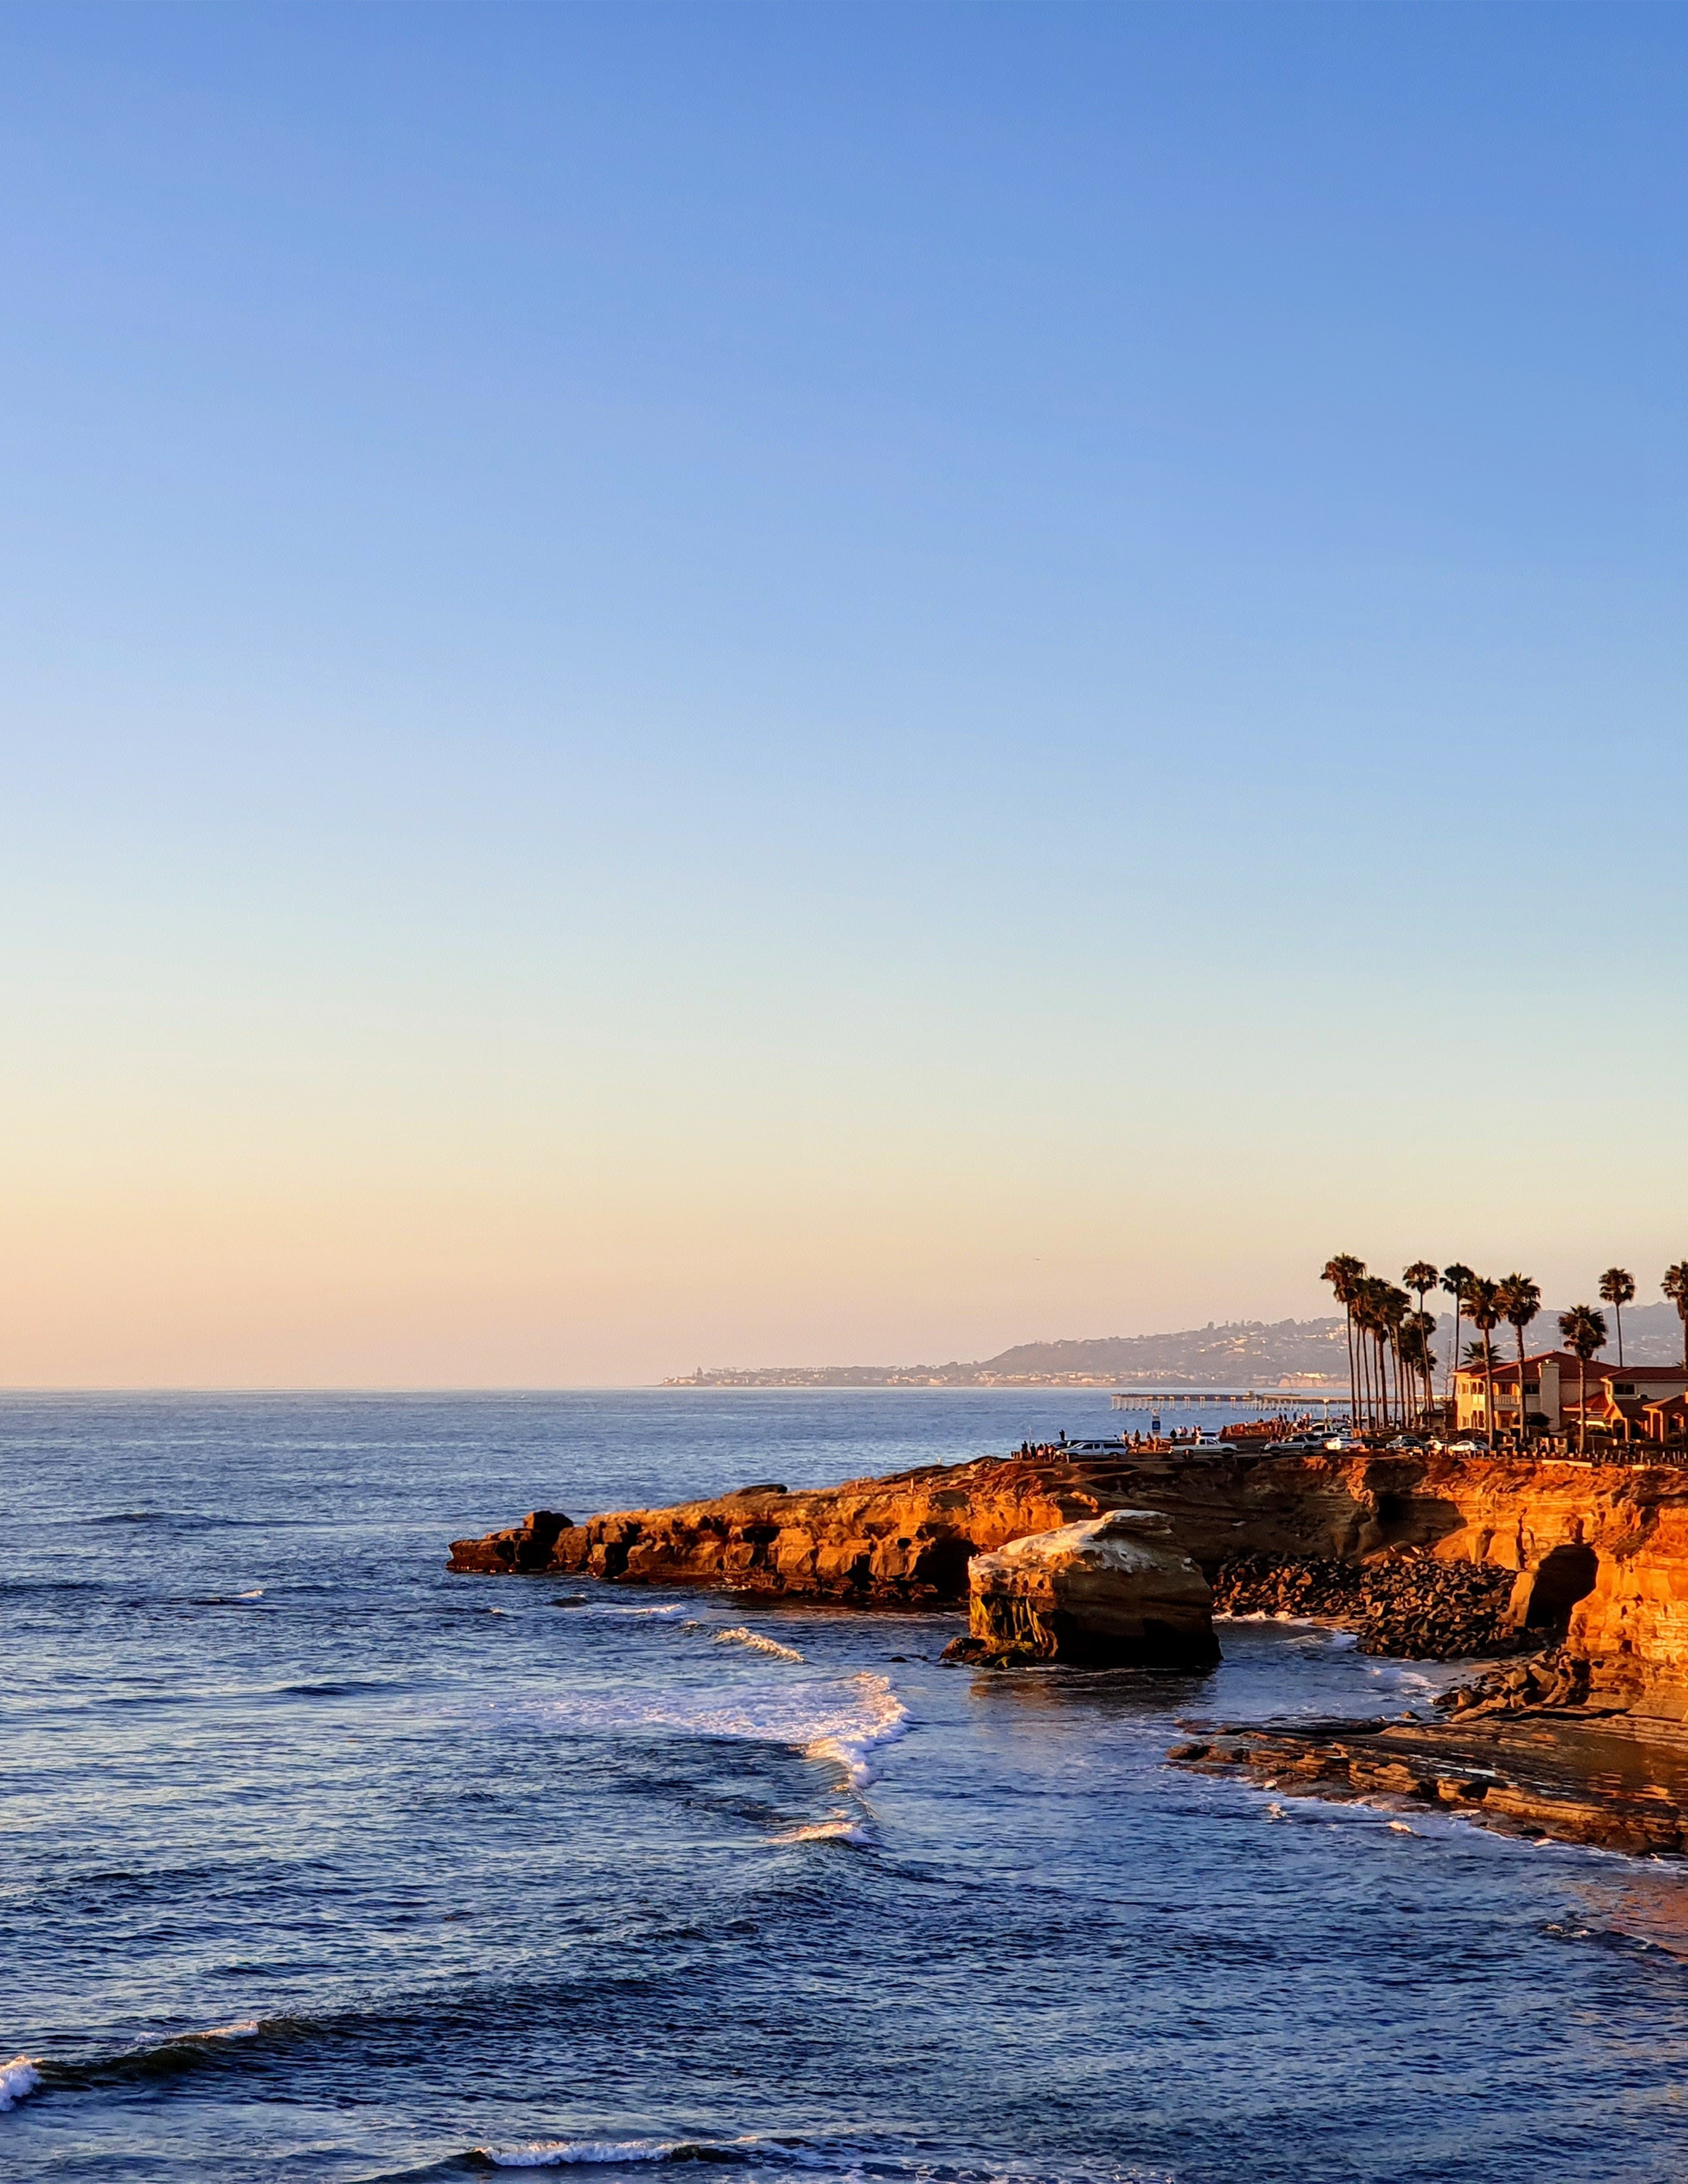
\includegraphics[width=\paperwidth]{images/background.png}}
    {
        \centering\fontfamily{phv}\selectfont
        {\Huge \bfseries Sentiment Analysis on Social Media Data for
            Brand Monitoring \par}
        \vspace{8pt}
        {\begin{center}
                \begin{tabular*}{\textwidth}{@{\extracolsep{\fill}}c c c}
                    {\LARGE Jonathan Agustin} &
                    {\LARGE Fernando Calderon} &
                    {\LARGE Juliet Lawton}
                \end{tabular*}
            \end{center}}
        \vspace{24pt}
        {\LARGE\bfseries \par}
    }
}

\pagenumbering{arabic}
\section{Introduction}

In the contemporary digital environment, companies are increasingly leveraging
social media platforms to track public perception of their brands. This
process, known as \textbf{Brand Identification} and \textbf{Sentiment
    Analysis}, employs \textbf{Natural Language Processing} (NLP), text analytics,
and computational linguistics to detect and extract subjective information
related to specific brands. This project, which intersects the fields of NLP,
\textbf{Deep Learning}, and \textbf{Classification}, aims to devise a model
that can accurately categorize social media posts into positive, negative, or
neutral sentiments towards specific brands, providing invaluable insights for
brand tracking.

\section{Problem Statement}

The task is to analyze sentiments towards brands from social media text data, a
complex and multifaceted classification problem. Given a set $X = \{x_1, x_2,
    \ldots, x_n\}$ of social media posts, our goal is to decipher the function $f:
    X \rightarrow Y$, where $Y = \{y_1, y_2, y_3\}$ represents the sentiment
labels, with $y_1 =$ positive, $y_2 =$ negative and $y_3 =$ neutral
respectively. This task requires a deep understanding of human language,
including context, sarcasm, and irony, which are often present in social media
posts. Machine Learning models, such as \textbf{BERT}, \textbf{RoBERTa}, and
\textbf{GPT-2}, are effective in understanding and leveraging context in
sentences, making them suitable for this task. However, the noisy nature of
social media text data, including misspellings, abbreviations, emojis, URLs,
and other non-alphanumeric characters, poses a significant challenge. The
problem statement is to develop a model that can accurately identify brands and
classify sentiments of a text as positive, negative, or neutral, extracted from
various social media sources. This task is crucial for businesses aiming to
track their brand sentiment in real-time, letting them respond promptly to
customer feedback and market trends. Despite the challenges posed by the
complexities of human language and the noisy nature of social media data, this
project aims to explore these nuances, address the obstacles, and strive for an
effective solution.

\section{Proposed Methodology}

We will use the Sentiment140 dataset from Stanford University, which includes
1.6 million tweets, for sentiment analysis. The dataset uses emoticons as a
proxy for sentiment labels, authentically representing sentiment in social
media text. For brand identification, we propose to use the Brand Sentiment
dataset from Surge AI, which includes over 1.5 million tweets mentioning over
2000 popular brands. Our methods are grounded on the robust capabilities of
pre-trained language models in response to the complex challenge of human
language understanding and brand identification. We will harness widely
recognized models from Hugging Face's model hub, such as BERT, DistilBERT,
RoBERTa, or GPT-2. These transformer-based models, constructed on the
foundation of large and diverse text corpora, provide a rich understanding of
language nuances and brand references. Our methods consist of three main
stages:

\begin{enumerate}
    \item \textbf{Data Preprocessing.} The first stage of our methods is Data
          Preprocessing, which involves transforming raw text into a structured format
          ready for modeling. This stage is crucial as it talks to social media data's
          inherent unstructuredness and noisiness, bridging the gap between
          human-generated content and machine-understandable language. We undertake
          certain preprocessing steps to ensure every piece of data feeds into our model
          in the most ideal form. The first step is \textbf{Noise Handling}, which
          removes irrelevant parts in our dataset, such as URLs, user handles, emojis,
          and non-alphanumeric characters. These parts rarely contribute to the broader
          understanding of sentiment and could introduce noise into our model. The second
          step is \textbf{Tokenization}, where we break down our text data into smaller
          units called tokens. These tokens, which correspond to words or subwords,
          represent the working units for our language models. They provide a granularity
          level at which our model learns the contextual relationship between different
          text parts.

    \item \textbf{Model Training.} The second stage involves the training and
          fine-tuning of our pre-trained language model on our processed dataset. We use
          the power of TensorFlow to ensure an efficient training process. Distinct from
          models trained from scratch, our chosen pre-trained models have undergone a
          phase of initial training on a vast corpus of text. They have captured the rich
          interplay of words and context in various linguistic scenarios.
          \textbf{Fine-tuning} refers to adjusting this pre-trained model's weights
          further, this time on our specific task. We thus align the model's capabilities
          to the nuances and features inherent to the sentiments in a social media text.

    \item \textbf{Model Evaluation.} The final stage evaluates our fine-tuned
          model's performance. Evaluation is crucial in measuring how successfully our
          model has learned to predict sentiments in the social media context. We use
          standard classification metrics: \textbf{Accuracy}, \textbf{Precision},
          \textbf{Recall}, and \textbf{F1 Score}. Accuracy gives us a measure of how
          correctly our model has classified the sentiments. Precision provides an
          understanding of how likely a positive prediction is positive. Recall tells us
          what proportion of actual positives is correctly classified. The F1 Score
          balances Precision and Recall and is best used when the class distribution is
          unbalanced. These metrics collectively provide a comprehensive view of our
          model's classification performance, enabling us to gauge its effectiveness and
          reliability.
\end{enumerate}

\section{Expected Behaviors/Outcomes}

\begin{itemize}
    \item \textbf{Model Performance.} The primary expectation is that our model
          will perform well in accuracy, precision, recall, and F1 score. These metrics
          will provide a comprehensive view of our model's performance. Accuracy will
          tell us how often our model is correct. Precision will inform us about the
          proportion of correct identifications. The recall will give us the ratio of
          actual positives that were identified correctly. The F1 score, the harmonic
          mean of precision and recall, will provide us with a metric that balances these
          considerations.

    \item \textbf{Understanding of Language Nuances and Brand Identification.}
          Beyond the quantitative metrics, we expect our model to show a nuanced
          understanding of human language and an ability to accurately identify brands.
          Given the complexity and ambiguity of human language, especially in social
          media posts, this is a non-trivial expectation. We expect our model to handle
          sarcasm, irony, and context-specific meanings common in social media posts, and
          correctly identify brand references within these posts.

    \item \textbf{Real-world Applicability.} Finally, we expect that our model
          will have real-world applicability. The ultimate goal of this project is to
          provide businesses with a tool to accurately and efficiently analyze sentiment
          from social media data. We expect that our model can provide actionable
          insights to help companies to make more informed decisions. For example, a
          business could use our model to track public sentiment about their brand in
          real-time, compare their performance with competitors based on public
          sentiment, or analyze customer feedback to improve their products or services.
\end{itemize}
\begin{thebibliography}{}

    \bibitem[Devlin et al., 2018]{devlin2018bert}
    Devlin, J., Chang, M. W., Lee, K., \& Toutanova, K. (2018).
    \newblock BERT: Pre-training of Deep Bidirectional Transformers for
    Language Understanding.
    \newblock {\em arXiv preprint arXiv:1810.04805}.

    \bibitem[Liu et al., 2019]{liu2019roberta}
    Liu, Y., Ott, M., Goyal, N., Du, J., Joshi, M., Chen, D., \ldots \&
    Stoyanov,
    V. (2019).
    \newblock RoBERTa: A Robustly Optimized BERT Pretraining Approach.
    \newblock {\em arXiv preprint arXiv:1907.11692}.

    \bibitem[Radford et al., 2019]{radford2019language}
    Radford, A., Wu, J., Child, R., Luan, D., Amodei, D., \& Sutskever, I.
    (2019).
    \newblock Language Models are Unsupervised Multitask Learners.
    \newblock {\em OpenAI Blog, 1(8)}.

    \bibitem[Sanh et al., 2019]{sanh2019distilbert}
    Sanh, V., Debut, L., Chaumond, J., \& Wolf, T. (2019).
    \newblock DistilBERT, a distilled version of BERT: smaller, faster, cheaper
    and lighter.
    \newblock {\em arXiv preprint arXiv:1910.01108}.

    \bibitem[Hutto \& Gilbert, 2014]{hutto2014vader}
    Hutto, C.J., \& Gilbert, E. (2014).
    \newblock VADER: A Parsimonious Rule-based Model for Sentiment Analysis of
    Social Media Text.
    \newblock {\em Eighth International Conference on Weblogs and Social Media
        (ICWSM-14). Ann Arbor, MI, June 2014}.

\end{thebibliography}

\thispagestyle{empty}

\end{document}
